% !TeX spellcheck = en_GB
%%%%%%%%%%%%%%%%%%%%%%%%%%%%%%%%%%%%%%%%%%%%%%%%%%%%%%%%%%%%%%%%%%%%%%%%%%%%%%%%
%\documentclass[handout]{beamer}\mode<handout>{\usetheme{default}}
%
%\documentclass[presentation]{beamer}\mode<presentation>{\usetheme{blackAMSBolognaFC}}
\documentclass[handout]{beamer}\mode<handout>{\usetheme{AMSBolognaFC}}
% \setbeamertemplate{bibliography item}{\insertbiblabel}
%%%%%%%%%%%%%%%%%%%%%%%%%%%%%%%%%%%%%%%%%%%%%%%%%%%%%%%%%%%%%%%%%%%%%%%%%%%%%%%%
\usepackage[english]{babel}
\usepackage[utf8]{inputenc}
%
\usepackage{magnini-ecai-2025-talk}
%%%%%%%%%%%%%%%%%%%%%%%%%%%%%%%%%%%%%%%%%%%%%%%%%%%%%%%%%%%%%%%%%%%%%%%%%%%%%%%%
\title[Learning \EL Terminologies from LLMs]{
    % same title of the presented paper
    Actively Learning \EL Terminologies
    \\
    from Large Language Models
}
%
% \subtitle{Extended Abstract}
%
% same authors order of the presented paper
\author[Magnini et al.]{
	\emph{Matteo Magnini}$^{*}$ % empth the presenting author
	\and 
	Riccardo Squarcialupi$^{*}$
	\\
	Martin T. Sterri$^{\dagger}$
	\and
	Ana Ozaki$^{\dagger,\ddagger}$
}
%
\institute[UniBo]{
    $^{*}$%Department of Computer Science and Engineering
    %\\
    \textsc{Alma Mater Studiorum} -- University of Bologna
    \\
    \texttt{
        \emph{matteo.magnini}@unibo.it, riccard.squarcialupi@studio.unibo.it
    }
    \vspace{.3cm}
    \\
    $^{\dagger}$University of Bergen
    \\
    \texttt{
        martin.sterri@student.uib.no, ana.ozaki@uib.no
    }
    \vspace{.3cm}
    \\
    $^{\ddagger}$University of Oslo
    \\
    \texttt{
        anaoz@ifi.uio.no
    }
}
%
\date[ECAI, 2025]{
	The European Conference on Artificial Intelligence (ECAI 2025)
	\\
	27 October, 2025, Bologna
}
%%%%%%%%%%%%%%%%%%%%%%%%%%%%%%%%%%%%%%%%%%%%%%%%%%%%%%%%%%%%%%%%%%%%%%%%%%%%%%%%
\AtBeginSection[]
{
%\\\\\\\\\\\\\\\\\\\\\
\begin{frame}<beamer>[c,noframenumbering]
\frametitle{Next in Line\ldots}
\tableofcontents[sectionstyle=show/shaded,subsectionstyle=hide]
\end{frame}
%\\\\\\\\\\\\\\\\\\\\\
}
\AtBeginSubsection[]
{
%\\\\\\\\\\\\\\\\\\\\\
\begin{frame}<beamer>[shrink,noframenumbering]
    \frametitle{Focus on\ldots}
	\mbox{~}
	\tableofcontents[currentsubsection,sectionstyle=shaded,subsectionstyle=show/shaded]
	\mbox{~}
\end{frame}
%\\\\\\\\\\\\\\\\\\\\\
}
%%%%%%%%%%%%%%%%%%%%%%%%%%%%%%%%%%%%%%%%%%%%%%%%%%%%%%%%%%%%%%%%%%%%%%%%%%%%%%%%
\begin{document}
%%%%%%%%%%%%%%%%%%%%%%%%%%%%%%%%%%%%%%%%%%%%%%%%%%%%%%%%%%%%%%%%%%%%%%%%%%%%%%%%

%\\\\\\\\\\\\\\\\\\\\\
\frame{\titlepage}
%\\\\\\\\\\\\\\\\\\\\\

%===============================================================================
\section{Motivation \& Context}
%===============================================================================

%\\\\\\\\\\\\\\\\\\\\\
\begin{frame}[c, allowframebreaks]{Context}

    \vfill
    
    The \alert{active learning} framework:
    %
    \vfill
    %
    \begin{itemize}
        \item a \alert{learner} attempts to learn some kind of \alert{knowledge};
        %
        \item by posing questions to a \alert{teacher};

        \vfill

        \item questions made by the learner are
        %
        \begin{itemize}
            \item \alert{membership} queries $\rightarrow$ ask whether \alert{concept inclusions} are true or false;
            %
            \item \alert{equivalence} queries $\rightarrow$ ask whether the idea od the learner about the knowledge of the teacher is correct or not.
        \end{itemize}
        
        \vfill
        
    \end{itemize}

    \framebreak

    \begin{figure}
        \centering
        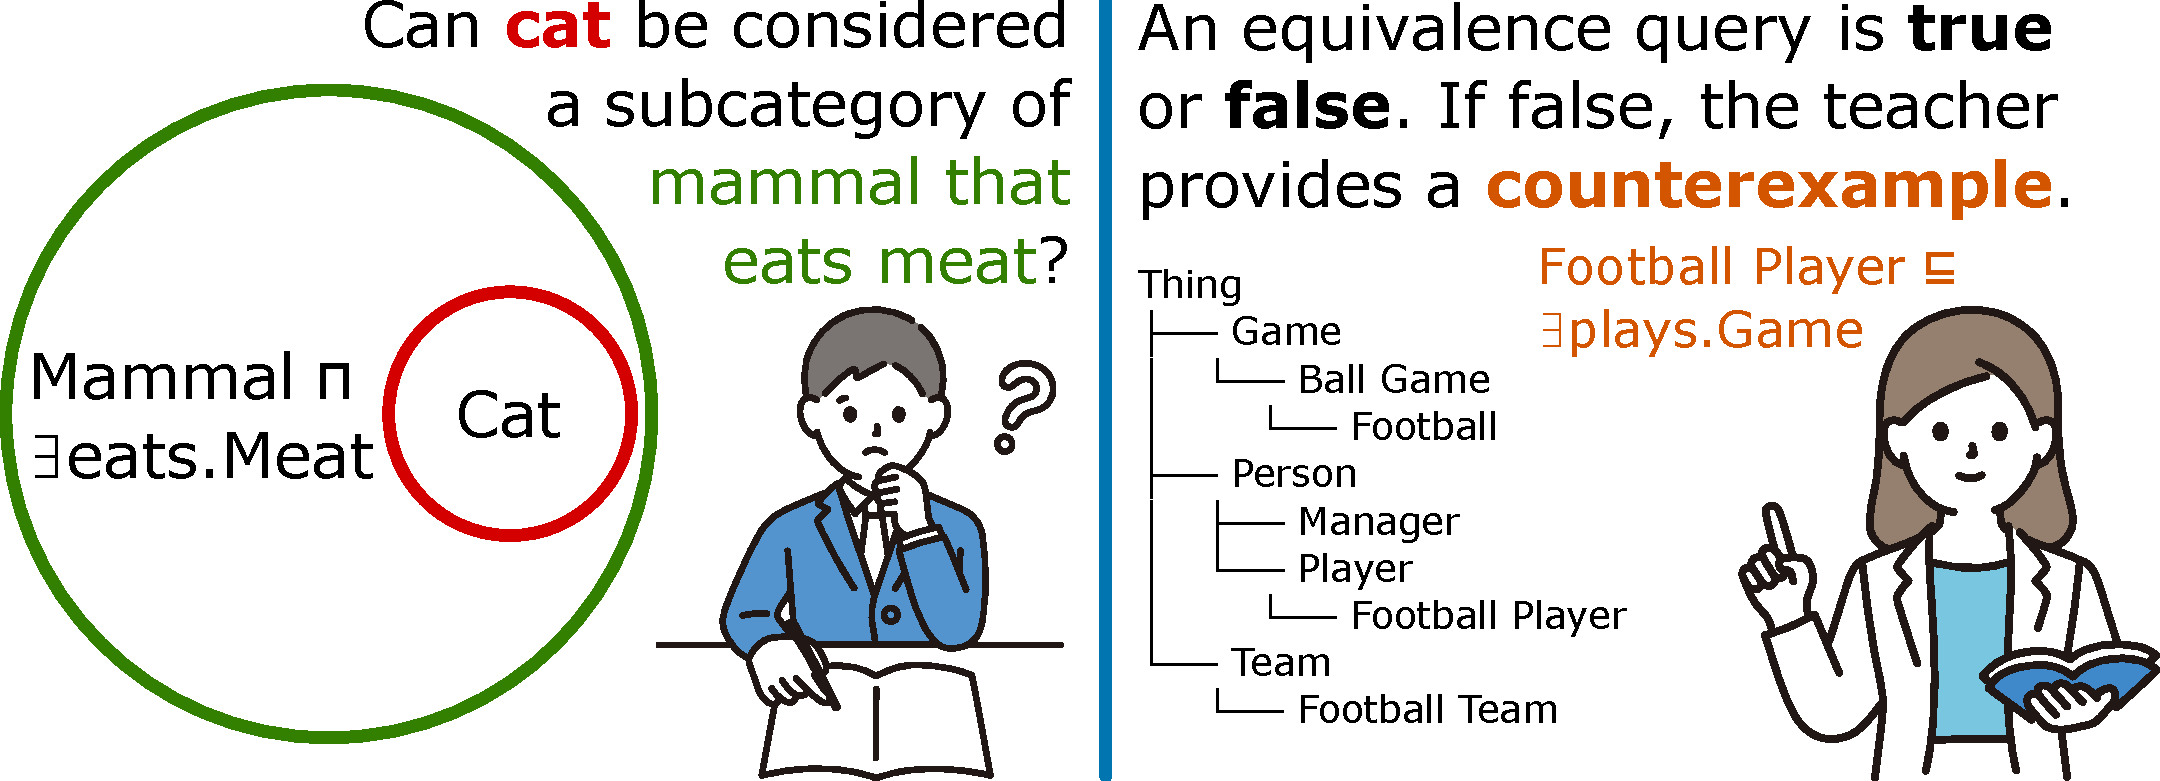
\includegraphics[width=0.8\textwidth]{figures/queries-example}
        \caption{Example of membership and equivalence queries}
        \label{}
    \end{figure}

    We want to use \alert{Large Language Models} (LLMs) as teachers in the \alert{Angluin}'s exact learning framework \ccite{DBLP:journals/ml/Angluin87}.

\end{frame}
%\\\\\\\\\\\\\\\\\\\\\

%\\\\\\\\\\\\\\\\\\\\\
\begin{frame}[c]{Motivation}
    Motivations for our work:
    %
    \vfill
    %
    \begin{itemize}
        \item to the best of our knowledge, the only implementation of the Angluin's exact learning framework uses a \alert{synthetic teacher} \ccite{DBLP:conf/kr/DuarteKO18};
        %
        \item ontology construction is a costly and time-consuming task that requires domain experts;
        %
        \item arguably, a boring and repetitive task for humans;
        %
        \item with LLMs as teachers, we can \alert{automate} the process of ontology construction;
        %
        \item with Angluin's framework, we build ontologies in a systematic way.
        %
    \end{itemize}
\end{frame}
%\\\\\\\\\\\\\\\\\\\\\


%===============================================================================
\section{Design}
%===============================================================================

%\\\\\\\\\\\\\\\\\\\\\
\begin{frame}[c, allowframebreaks]
\frametitle{Algorithm}

    \begin{figure}
        \centering
        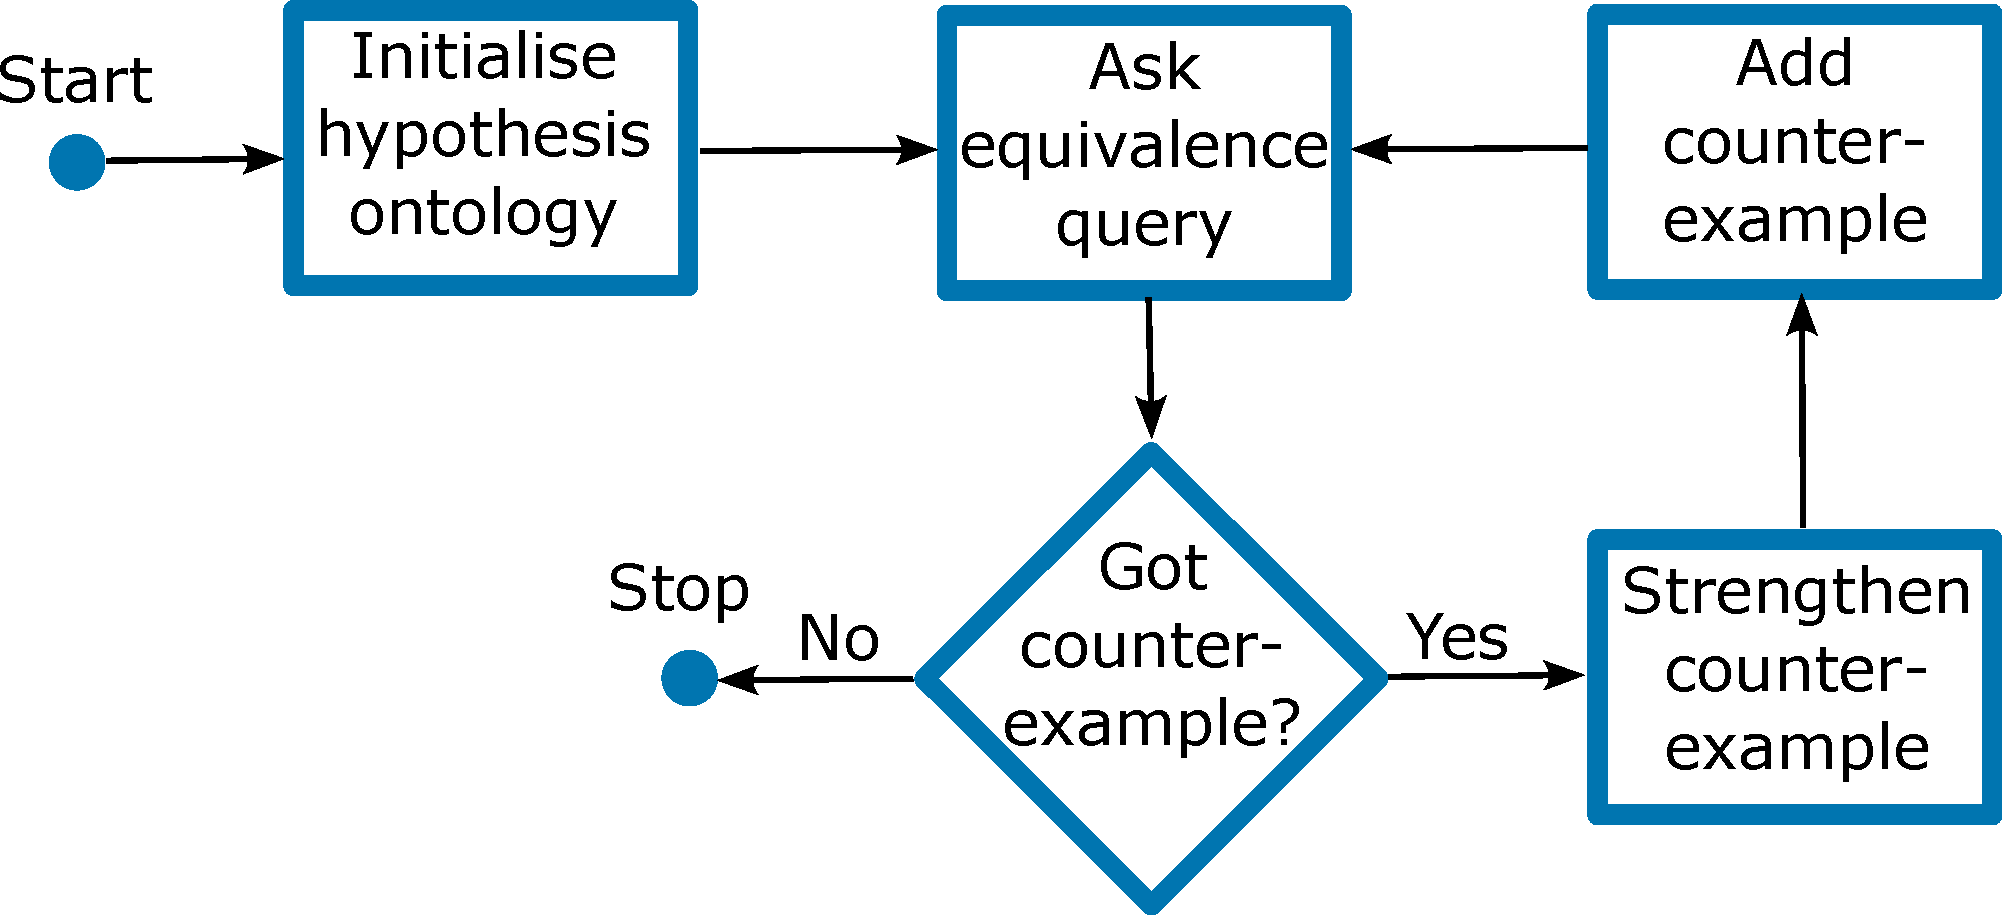
\includegraphics[width=0.8\textwidth]{figures/algorithm}
        \caption{Overview of the exact learning algorithm.}
        \label{fig:algorithm}
    \end{figure}

    \framebreak

%    \vfill

    Equivalence query are \alert{symulated} via random \alert{sampling}.
    %
    The algorithm checks if the classification of the examples match with the information in the hypothesis:

    \begin{itemize}
        %
        \item true inclusions must be \alert{logical consequences};
        %
        \item false ones must not.
        %
    \end{itemize}

%    \vfill

    If the hypothesis fits the classification of the concept inclusions, learning stops.
    Otherwise, the inclusion not fitting the hypothesis is used as a \alert{counterexample}.

%    \vfill

    \framebreak

    The sampling-based simulation can yield \alert{PAC} \ccite{DBLP:journals/cacm/Valiant84} guarantees when the sample size

    \begin{equation*}
        \lvert S \rvert \geq \frac{\ln\left(\lvert H \rvert / \gamma\right)}{\epsilon}
    \end{equation*}

    is computed from the hypothesis space $H$ (\EL terminologies of bounded structure) and parameters $\epsilon$ (error) and $\gamma$ (confidence).


\end{frame}
%\\\\\\\\\\\\\\\\\\\\\

%\\\\\\\\\\\\\\\\\\\\\
\begin{frame}[c, allowframebreaks]
\frametitle{Learner's operations}

    When the teacher replies with a counterexample, the learner before adding it to the hypothesis \alert{processes} it.
    The learner performs operations, that use membership queries, in order to \alert{maximise} how informative the concept inclusions are and also to \alert{minimise} their size.

    \begin{itemize}
        \item Decompose Left
        \item Decompose Right
        \item Merging
        \item Branching
        \item Saturation
        \item Desaturation
    \end{itemize}

    \framebreak

    Decompose Right

    \begin{columns}[c]
    \column{0.55\textwidth}
    \vspace{-1cm}
    \begin{equation*}
    \begin{aligned}
        T &= \{A \sqsubseteq \exists r.\top,\; B \sqsubseteq \exists r.\top,\; A \sqsubseteq B\} \\
        H &= \{A \sqsubseteq B\} \\
        \text{C} &= A \sqsubseteq
            \textcolor{blue}{B \sqcap}
            \textcolor{orange}{\exists s.\top}
            \textcolor{blue}{\sqcap}
            \textcolor{green}{\exists r.\top}
        \\[0.8em]
        &\Downarrow \\[0.8em]
        \text{C} &= \textcolor{blue}{B} \sqsubseteq
            \textcolor{orange}{\exists s.\top}
    \end{aligned}
    \end{equation*}

    \column{0.45\textwidth}
    \centering

    \vspace{1cm}

    \begin{tikzpicture}[
      every node/.style={
        draw, rounded corners=4pt,
        minimum width=1.6cm, minimum height=0.8cm,
        align=center, thick
      },
      root/.style={draw=blue},
      leftchild/.style={draw=orange!90!black},
      rightchild/.style={draw=green!60!black},
      arrow/.style={->, very thick, shorten >=2pt, shorten <=2pt}
    ]
        \node[root] (root) {\{$B$\}};
        \node[leftchild, below left=0.7cm and 0.1cm of root] (left) {\{\}};
        \node[rightchild, below right=0.7cm and 0.1cm of root] (right) {\{\}};
        \draw[arrow, orange!90!black] (root) -- (left)
            node[midway, above left=-0.1cm, text=black, font=\small, fill=none, draw=none] {$s$};
        \draw[arrow, green!60!black] (root) -- (right)
            node[midway, above right=-0.1cm, text=black, font=\small, fill=none, draw=none] {$r$};
    \end{tikzpicture}

    \vspace{1cm}

    \begin{tikzpicture}[
      every node/.style={
        draw, rounded corners=4pt,
        minimum width=1.6cm, minimum height=0.8cm,
        align=center, thick
      },
      root/.style={draw=black},
      leftchild/.style={draw=orange!90!black},
      rightchild/.style={draw=black},
      arrow/.style={->, very thick, shorten >=2pt, shorten <=2pt}
    ]
        \node[root] (root) {\{$B$\}};
        \node[leftchild, below left=0.7cm and 0.1cm of root] (left) {\{\}};
        \node[rightchild, below right=0.7cm and 0.1cm of root] (right) {\{\}};
        \draw[arrow, orange!90!black] (root) -- (left)
            node[midway, above left=-0.1cm, text=black, font=\small, fill=none, draw=none] {$s$};
        \draw[arrow, black] (root) -- (right)
            node[midway, above right=-0.1cm, text=black, font=\small, fill=none, draw=none] {$r$};
    \end{tikzpicture}

    \end{columns}
\end{frame}

%\\\\\\\\\\\\\\\\\\\\\

\section{Validation}

%\\\\\\\\\\\\\\\\\\\\\
\begin{frame}[c,allowframebreaks]
\frametitle{Ontologies}

    \begin{table}[]
        \centering
        \resizebox{\columnwidth}{!}{
            \begin{tabular}{|l|c|c|c|c|c|}
                \hline
                \textbf{Ontology} & \textbf{$\NC$} & \textbf{$\NR$} & \textbf{Log. Ax.} & \textbf{PAC Sample} & \textbf{Poss. Ax.} \\
                \hline
                \rowcolor[HTML]{EFEFEF}
                Animals & 17 & 4 & 12 & 542 & 6,936\\
                \hline
                \rowcolor[HTML]{FFFFFF}
                Cell & 22 & 0 & 24 & 1,119 & 10,164\\
                \hline
                \rowcolor[HTML]{EFEFEF}
                Football & 10 & 3 & 9 & 341 & 1,500\\
                \hline
                \rowcolor[HTML]{FFFFFF}
                Generations & 20 & 4 & 18 & 847 & 10,800\\
                \hline
                \rowcolor[HTML]{EFEFEF}
                University & 7 & 3 & 4 & 139 & 588\\
                \hline
            \end{tabular}
        }
        \caption{Ontology statistics and PAC sample sizes with $\epsilon=0.2$ and $\gamma=0.1$. $\NC$ and $\NR$ are the number of concept and role names occurring in the ontologies.}
        \label{tb:small-ontologies}
    \end{table}

    \framebreak

    \begin{table}[]
    \centering
    \resizebox{0.9\columnwidth}{!}{ % Reduced size slightly
    \begin{tabular}{|l|c|c|c|c|c|}
        \hline
        \textbf{Ontology} & \textbf{\NC} & \textbf{\NR} & \textbf{Log. Ax.} & \textbf{PAC Sample}  & \textbf{Pos. Ax.}  \\
        \hline
        \rowcolor[HTML]{EFEFEF}
        Ab. Elb. J. C. & 27 & 14 & 43 & 2,286 & 39,366\\
        \hline
        \rowcolor[HTML]{FFFFFF}
        BNF Sec. & 36 & 24 & 80 & 4,646 & 107,568\\
        \hline
        \rowcolor[HTML]{EFEFEF}
        Chlorhexidine & 23 & 14 & 38 & 1,946 & 26,450\\
        \hline
        \rowcolor[HTML]{FFFFFF}
        Cone of Tissue & 42 & 42 & 100 & 6,163 & 220,500\\
        \hline
        \rowcolor[HTML]{EFEFEF}
        Kalli Krein & 18 & 10 & 27 & 1,279 & 11,988\\
        \hline
        \rowcolor[HTML]{FFFFFF}
        Neon & 16 & 10 & 25 & 1,149 & 8,960\\
        \hline
        \rowcolor[HTML]{EFEFEF}
        Pin & 43 & 40 & 99 & 6,113 & 225,578\\
        \hline
        \rowcolor[HTML]{FFFFFF}
        Pros. Drug & 29 & 14 & 47 & 2,540 & 47,096\\
        \hline
        \rowcolor[HTML]{EFEFEF}
        Zopiclone & 32 & 36 & 77 & 4,465 & 105,472\\
        \hline
        \rowcolor[HTML]{FFFFFF}
        Zuccini & 33 & 22 & 58 & 3,295 & 82,764\\
        \hline
    \end{tabular}
    }
    \caption{Ontology statistics and PAC sample sizes with $\epsilon=0.2$ and $\gamma=0.1$ for medical ontologies (sub modules of the Galen ontology \ccite{Rector2008TheGH}).}
    \label{tb:modules-ontologies}
\end{table}

\end{frame}
%\\\\\\\\\\\\\\\\\\\\\

%\\\\\\\\\\\\\\\\\\\\\
\begin{frame}[c,allowframebreaks]
\frametitle{LLMs and how to query them}

    $\textcolor{blue}{\text{Cat}} \sqsubseteq \textcolor{green}{\text{Mammal}} \sqcap \textcolor{orange}{\exists \text{eats.Meat}}$

    \begin{itemize}
        \item Manchester OWL Syntax
        \begin{itemize}
            \item \textcolor{blue}{Cat} SubClassOf \textcolor{green}{\text{Mammal}} and \textcolor{orange}{eats some Meat}?
        \end{itemize}
        \item Natural Language
        \begin{itemize}
            \item Can \textcolor{blue}{Cat} be considered a subcategory of ``\textcolor{green}{\text{Mammal}} that is also \textcolor{orange}{something that eats some Meat}''?
        \end{itemize}
    \end{itemize}

    \vspace{1cm}

    LLMs used as teachers:

    \begin{itemize}
        \item Llama2 (13B)
        \item Llama3 (8B)
        \item Mistral (7B)
        \item Mixtral (47B)
    \end{itemize}

    \framebreak

    Two different system prompts used to query the LLMs:
    \begin{itemize}
        \item Concise:
        \begin{itemize}
            \item Answer with only True or False.
        \end{itemize}
        \item Detailed:
        \begin{itemize}
            \item You need to classify the following statements as True or False.
            The statement will be provided in either Manchester OWL syntax or natural language.
            Strictly follow these guidelines:\\
            1. answer with only True or False;\\
            2. entities with has part relation are not in a subclass relation;\\
            3. take a deep breath before answering;\\
            4. if you are unsure about the classification, answer with False.
        \end{itemize}
    \end{itemize}

\end{frame}

%\\\\\\\\\\\\\\\\\\\\\

\begin{frame}[c,allowframebreaks]
\frametitle{Evalualtion}

    \vfill

    The metrics are computed considering all possible axioms of the form:
    %
    \begin{itemize}
        \item $A \sqsubseteq B$
        \item $A \sqcap B \sqsubseteq C$
        \item $B \sqsubseteq \exists r.A$
        \item $\exists r.A \sqsubseteq B$
    \end{itemize}

    \vfill

    These axioms are formulated with a finite signature. Tautologies, such as:
    %
    \begin{itemize}
        \item $A \sqsubseteq A$
        \item $A \sqcap B \sqsubseteq B$
        \item $A \sqcap B \sqsubseteq A$
    \end{itemize}
    %
    are removed to avoid artificially inflating true positives.

    \vfill

    \framebreak

    Axioms are classified as:
    %
    \begin{itemize}
        \item \alert{TP} Entailed by both the original and learnt ontology;
        \item \alert{TN} Not entailed by either ontology;
        \item \alert{FN} Entailed by the original ontology but not the learnt one;
        \item \alert{FP} Entailed by the learnt ontology but not the original one.
    \end{itemize}

\end{frame}
%\\\\\\\\\\\\\\\\\\\\\

%\\\\\\\\\\\\\\\\\\\\\
\begin{frame}[c,allowframebreaks]
    \frametitle{Results}

    \begin{table}[]
    \centering
    \resizebox{0.7\columnwidth}{!}{
    \begin{tabular}{|l|c|c|c|c|}
    \hline
    \textbf{Ontology} & \textbf{Accuracy} & \textbf{Recall} & \textbf{Precision} & \textbf{F1-Score} \\
    \hline
    \rowcolor[HTML]{EFEFEF}
    Animals & 0.737 & 0.858 & 0.381 & 0.428 \\
    \hline
    \rowcolor[HTML]{FFFFFF}
    Cell & 0.391 & 0.733 & 0.206 & 0.284 \\
    \hline
    \rowcolor[HTML]{EFEFEF}
    Football & 0.553 & 0.89 & 0.422 & 0.477 \\
    \hline
    \rowcolor[HTML]{FFFFFF}
    Generations & 0.691 & 0.658 & 0.564 & 0.476 \\
    \hline
    \rowcolor[HTML]{EFEFEF}
    University & 0.622 & 0.629 & 0.313 & 0.302 \\
    \hline
    \end{tabular}}
    \caption{Results of ExactLearner+LLM grouped by ontologies.}
    \label{tb:results-small-ontologies}
    \end{table}

    \begin{table}[]
    \centering
    \resizebox{0.7\columnwidth}{!}{
    \begin{tabular}{|l|c|c|c|c|}
    \hline
    \textbf{Model} & \textbf{Accuracy} & \textbf{Recall} & \textbf{Precision} & \textbf{F1-Score} \\
    \hline
    \rowcolor[HTML]{EFEFEF}
    Llama2 (13b) & 0.521 & 0.71 & 0.294 & 0.314 \\
    \hline
    \rowcolor[HTML]{FFFFFF}
    Llama3 (8b) & 0.43 & 0.947 & 0.218 & 0.333 \\
    \hline
    \rowcolor[HTML]{EFEFEF}
    Mistral (7b) & 0.741 & 0.747 & 0.45 & 0.49 \\
    \hline
    \rowcolor[HTML]{FFFFFF}
    Mixtral (47b) & 0.705 & 0.611 & 0.547 & 0.436 \\
    \hline
    \end{tabular}}
    \caption{Results of ExactLearner+LLM grouped by models.}
    \label{tb:results-small-models}
    \end{table}

    \framebreak

    \begin{table}[]
    \centering
    \resizebox{0.7\columnwidth}{!}{
    \begin{tabular}{|l|c|c|c|c|}
    \hline
    \textbf{Prompt Type} & \textbf{Accuracy} & \textbf{Recall} & \textbf{Precision} & \textbf{F1-Score} \\
    \hline
    \rowcolor[HTML]{EFEFEF}
    M. OWL Syntax & 0.34 & 0.93 & 0.165 & 0.262 \\
    \hline
    \rowcolor[HTML]{FFFFFF}
    Natural Language & 0.751 & 0.811 & 0.414 & 0.511 \\
    \hline
    \rowcolor[HTML]{EFEFEF}
    A. M. OWL Syntax & 0.537 & 0.767 & 0.326 & 0.347 \\
    \hline
    \rowcolor[HTML]{FFFFFF}
    A. Natural Language & 0.767 & 0.506 & 0.603 & 0.454 \\
    \hline
    \end{tabular}}
    \caption{Results of ExactLearner+LLM grouped by prompts.}
    \label{tb:results-small-prompt}
    \end{table}

    \framebreak

    \begin{figure}
        \centering
        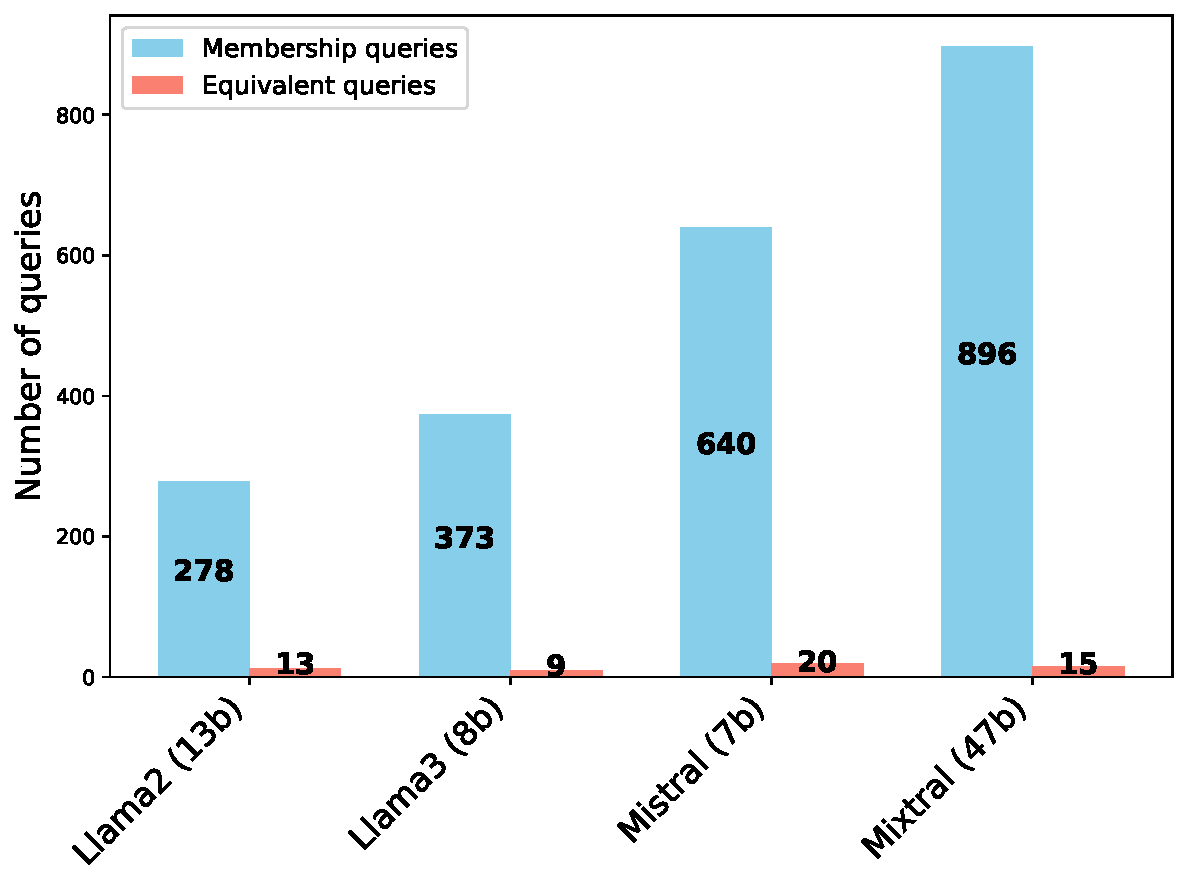
\includegraphics[width=0.5\textwidth]{figures/query_counts}
        \caption{Average number of membership and (simulated) equivalence queries grouped by LLM.}
        \label{fig:query-counts}
    \end{figure}

    \framebreak

    \begin{figure}
      \centering
      \begin{minipage}{0.6\textwidth}
        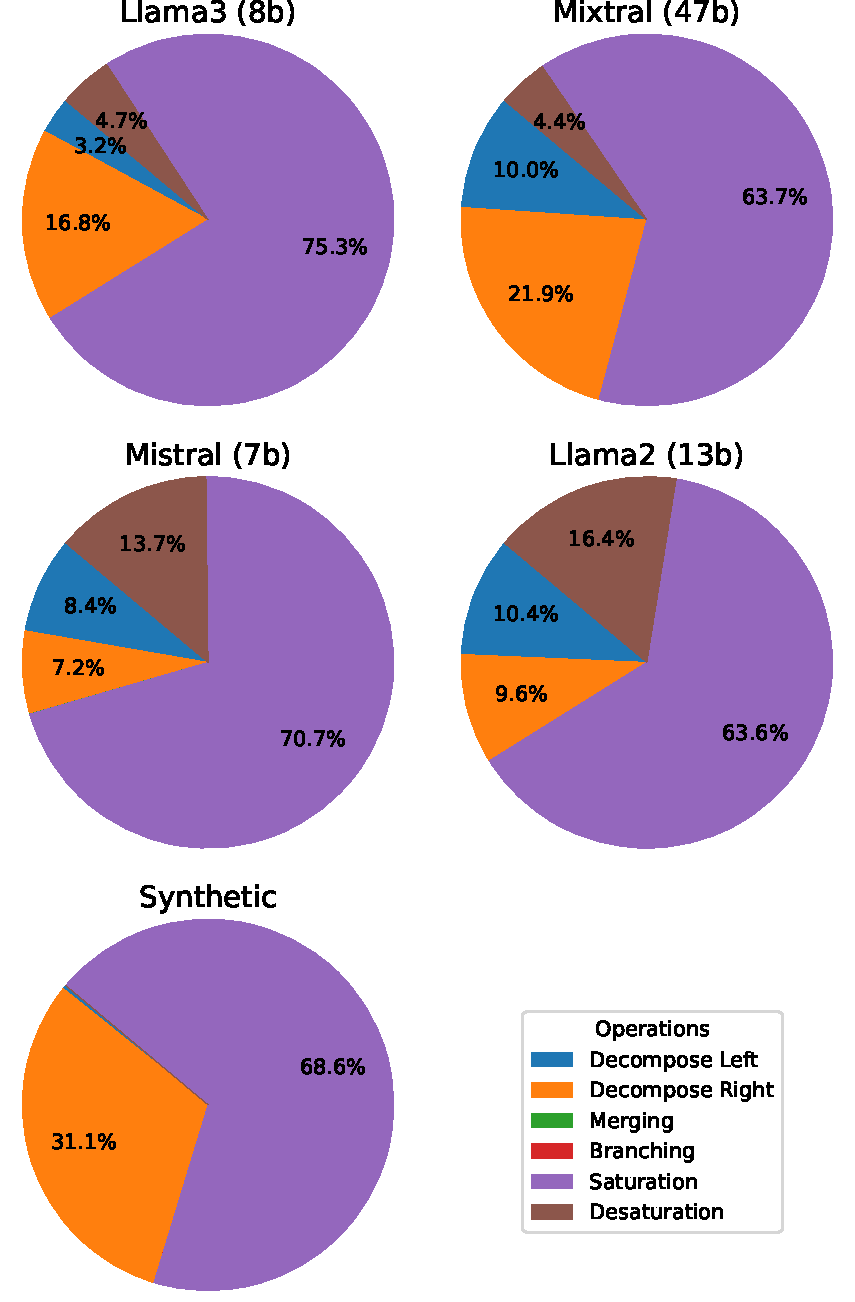
\includegraphics[width=0.6\linewidth]{figures/operations}
      \end{minipage}%
      \hspace{-1cm}
      \begin{minipage}{0.3\textwidth}
        \captionof{figure}{Aggregated results of the operations performed by the learner during the PAC learning of all the ontologies grouped by teacher type (LLMs and synthetic).}
          \label{fig:operations}
      \end{minipage}
    \end{figure}

\end{frame}


%===============================================================================
\section*{}
%===============================================================================
\frame{\titlepage}

%===============================================================================
\section*{\bibname}
%===============================================================================

\setbeamertemplate{page number in head/foot}{}
%\\\\\\\\\\\\\\\\\\\\\
\begin{frame}[t,allowframebreaks,noframenumbering]\frametitle{\refname}
% \begin{frame}[c]\frametitle{\refname}
	\footnotesize
%	\scriptsize
    \bibliographystyle{apalike-AMS}
    % \bibliographystyle{plain}
	\bibliography{magnini-ecai-2025-talk}
\end{frame}
%\\\\\\\\\\\\\\\\\\\\\

%%%%%%%%%%%%%%%%%%%%%%%%%%%%%%%%%%%%%%%%%%%%%%%%%%%%%%%%%%%%%%%%%%%%%%%%%%%%%%%%
\end{document}
%%%%%%%%%%%%%%%%%%%%%%%%%%%%%%%%%%%%%%%%%%%%%%%%%%%%%%%%%%%%%%%%%%%%%%%%%%%%%%%%
